\documentclass[a4paper,14pt]{extreport} %размер бумаги устанавливаем А4, шрифт 14пунктов
\usepackage[T2A]{fontenc}
\usepackage{booktabs} % For prettier tables
\usepackage[utf8]{inputenc}%включаем свою кодировку: koi8-r или utf8 в UNIX, cp1251 в Windows
\usepackage[english,russian]{babel}%используем русский и английский языки с переносами
\usepackage{amssymb,amsfonts,amsmath,mathtext,cite,enumerate,float} %подключаем нужные пакеты расширений
\usepackage[dvips]{graphicx}
\usepackage{pgfplots}
%\usepackage{listings}
\usepackage[linesnumbered,boxed]{algorithm2e}
\graphicspath{{./images/}}%путь к рисункам


\makeatletter
\renewcommand{\@biblabel}[1]{#1.} % Заменяем библиографию с квадратных скобок на точку:
\makeatother

\usepackage{extsizes}

\usepackage{geometry} % Меняем поля страницы
\geometry{left=3cm}% левое поле
\geometry{right=2cm}% правое поле
\geometry{top=2cm}% верхнее поле
\geometry{bottom=2cm}% нижнее поле
\linespread{1.3}

%\renewcommand{\theenumi}{\arabic{enumi}}% Меняем везде перечисления на цифра.цифра
%\renewcommand{\labelenumi}{\arabic{enumi}}% Меняем везде перечисления на цифра.цифра
%\renewcommand{\theenumii}{.\arabic{enumii}}% Меняем везде перечисления на цифра.цифра
%\renewcommand{\labelenumii}{\arabic{enumi}.\arabic{enumii}.}% Меняем везде перечисления на цифра.цифра
%\renewcommand{\theenumiii}{.\arabic{enumiii}}% Меняем везде перечисления на цифра.цифра
%\renewcommand{\labelenumiii}{\arabic{enumi}.\arabic{enumii}.\arabic{enumiii}.}% Меняем везде перечисления на цифра.цифра


\begin{document}
\begin{titlepage}
\newpage

\begin{center}
\small МИНИСТЕРСТВО ОБРАЗОВАНИЯ И НАУКИ РОССИЙСКОЙ ФЕДЕРАЦИИ \\
\vspace{1cm}
\small ФЕДЕРАЛЬНОЕ ГОСУДАРСТВЕННОЕ АВТОНОМНОЕ ОБРАЗОВАТЕЛЬНОЕ \\*
\small УЧРЕЖДЕНИЕ ВЫСШЕГО ОБРАЗОВАНИЯ \\*
\small "МОСКОВСКИЙ ФИЗИКО-ТЕХНИЧЕСКИЙ ИНСТИТУТ \\*
\small (ГОСУДАРСТВЕННЫЙ УНИВЕРСИТЕТ)" \\*
\vspace{1cm}
\small ФАКУЛЬТЕТ ИННОВАЦИЙ И ВЫСОКИХ ТЕХНОЛОГИЙ \\*
\small КАФЕДРА ТЕОРЕТИЧЕСКИХ И ПРИКЛАДНЫХ ПРОБЛЕМ ИННОВАЦИЙ \\*
\hrulefill
\end{center}

\vspace{4em}

\begin{center}
\textbf{ВЫПУСКНАЯ КВАЛИФИКАЦИОННАЯ РАБОТА} \\
\vspace{1em}
\small \textbf{(МАГИСТЕРСКАЯ РАБОТА)} \\
\vspace{1em}
\small \textbf{Направление подготовки: 03.04.01 "Прикладные математика и физика"} \\
\vspace{1em}
\textsc{\textbf{НА ТЕМУ:}} \\
\vspace{2em}
\large \textsc{\textbf{Единая автоматизированная информационная система поддержки и сопровождения проектов, созданных с применением стандарта BIM}}
\end{center}

\vspace{6em}

\begin{flushleft}
Студент \hrulefill Княжев В.А. \\
\vspace{1em}
Научный руководитель \hrulefill Зырин С.В.\\
\vspace{1em}
%Рецензент \\
%к.ф.-м.н., в.н.с. АБВГ \hrulefill Петров В.В.\\
%\vspace{1.5em}
%Зав. кафедрой  ХХХ \\
%д.ф-м.н, профессор \hrulefill Сидоров Г.Г.
\end{flushleft}

\vspace{\fill}

\begin{center}
г. Москва, 2019
\end{center}

\end{titlepage}% это титульный лист
\tableofcontents % это оглавление, которое генерируется автоматически

\newpage
\chapter{Введение}
\section{Актуальность проблемы}

Темпы строительства зданий и промышленных объектов в мире и сложность конструкций увеличивается с каждым годом \cite{BUILDING_GROWTH_RATE}. Ранее использовавшиеся методы проектирования чертежей на бумаге отходят на второй план, и все более активно используются компьютерные технологии \cite{BUILDING_SOFTWARE}, а также становится очевидной необходимость повсеместного введения стандартов проектирования зданий. \\
Одним из наиболее современных стандартов проектирования является стандарт BIM (Building Information Modeling)\cite{BIM_FUTURE}. Его концепция позволяет не только проектировать здания, но также охватить весь их жизненный цикл: от управления затратами и строительством здания до его эксплуатации. \\
Подобная всеобъемлемость хороша тем, что вся информация о конструкции содержится в одном проекте. Это помогает сохранять целостность данных, позволяет быстрее выявлять ошибки и уменьшать стоимость ремонта. Но также из этого вытекает необходимость координации одновременной работы большого количества людей над одним проектом: крупных команд архитекторов, иногда распределенных по всему миру, эксплуатирующих организаций и всех других людей, участвующих в обслуживании здания. \\
Поэтому очень важно иметь возможность одновременного изменения BIM представления объекта разными людьми без потери каких-либо данных. Но малейшая ошибка в одном из элементов конструкции, не обнаруженная вовремя, может привести к серьезным последствиям, например к дополнительным затратам на проект. Поэтому важно в любой момент времени иметь доступ к электронному журналу аудита всех изменений проекта. \\

TODO добавить предложение для перехода в постановке задачи


\newpage 
\section{Постановка задачи}

Требуется разработать веб-систему, которая бы могла предоставить пользователям следующие возможности:
\begin{enumerate}
\item Управление жизненным циклом проектов. \\
Создание проекта, добавление, редактирование  и удаление файлов, управление правами доступа к проекту.
\item Отслеживание изменений проекта во времени. \\
Отображение списка всех изменений проекта, а также возможность просмотра версии данных или внесенных в проект изменений в конкретный момент времени.
\item Одновременное внесение изменений в проекты несколькими пользователями. \\
Пользователи могут работать над разными частями проекта в одно и то же время. При наличии конфликтующих изменений предоставляется возможность сохранения изменений, внесенных как другими пользователями, так и текущим.
\item Подготовка окружения, запуск системы и ее масштабируемость. \\
Возможность быстрой подготовки окружения и запуска сервиса для мговенного развертывания веб-платформы. В моменты пиковой нагрузки пользователей, веб-платформа не должна терять производительность.
\end{enumerate}

\newpage

\chapter{Основная часть}
\section{Стандарт BIM}

BIM (Building Information Modeling или информационное моделирование здания) - это стандарт создания проектов строительных объектов, с учетом физических и функциональных характеристик. В основе проектов, созданных по этому стандарту, лежит информация о каждом из создаваемых объектов. \\
Исторически, компьютерные проекты зданий были просто цифровыми аналогами бумажных чертежей, которые использовались архитекторами, дизайнерами, инженерами и строительными бригадами. 
Это крайне неэффективный способ планирования строительства, потому что разные команды должны получать доступ к информации проекта по-разному, часто в разное время на протяжении всего проекта. \\
Архитекторам нужны «чертежи» - планы, разрезы и фасады. Дизайнерам интерьера нужны 3D модели. Строителям и инженерам нужно третье. Если использовать стандартные подходы к планированию, необходимо затратить время специалистов на графическую конвертацию архитектурного чертежа в необходимый формат. Любые внесенные в архитектурный проект изменения должны распространяться по каждому файлу вручную, и затем проверяться на правильность. \\
При данной схеме проектирование здания становится трудоемким итеративным процессом без единого источника информации об объекте, и соответственно с большой вероятностью ошибок и несоответствий между версиями разных специалистов. \\
BIM позволяет решать эти проблемы: на передний план выходит не графическое представление, а информация о каждом из объектов в будущем здании, а затем уже эти данные представляются графически. \\
В общем, объект BIM - это любой аспект здания, который не является частью информации о материалах строительства. Объекты BIM подразделяются на два типа: составные и слоистые.
\begin{itemize}
\item составные объекты \\
Имеют фиксированные очертания и размеры. Это могут быть окна, двери, трубопроводы, воздуховоды, электромонтажные работы и т. д.
\item слоистые объекты \\
Не имеют фиксированных форм или размеров и включают в себя большинство конструктивных элементов, таких как кровля, стены и потолки.
\end{itemize}
С практической точки зрения объекты BIM далее подразделяются на общие и частные объекты. Общие объекты содержатся в библиотеках объектов, общих для большинства программ BIM, и используются на начальном этапе проектирования. Частные объекты - это объекты, которые отражают характеристики конкретных коммерческих продуктов, которые будут использоваться в строительстве. Как правило, они создаются для каждого проекта индивидуально. \\
Входные данные о конструкции и дизайне, состоящие из объектов BIM, могут быть сделаны через графический интерфейс. Информация о разных сферах проекта хранится отдельно, но может быть сгенерирована в любом количестве форматов. \\
Подобная структура проектов, созданных по стандарту BIM, предоставляет возможности для работы нескольких команд, которые могут физически находиться в разных частях света, одновременно над одним проектом \cite{BIM_ADVANTAGES}. Автоматическая и простая конвертация из одного формата в другой позволяет сокращать трудозатраты специалистов и соответственно облегчает взаимодействие между несколькими командами. \\
Существует несколько уровней зрелости стандарта BIM:
\begin{enumerate}
\item Уровень 0 BIM \\
Фактически означает только 2D чертеж и отсутствие коллаборации. Распространение проекта между группами осуществляется через бумажные или электронные версии.
\item Уровень 1 BIM \\
На этом уровне 3D модели используются для визуализации концепции, и 2D чертежи для разработки строительной документации. Обмен информацией осуществляется через общую среду данных, которая обычно обеспечивается заказчиком.
\item Уровень 2 BIM \\
Представляет собой комплексную модель, работа над которой ведется специалистами из разных областей деятельности в различных программах. Сборка общей модели данных, ее анализ и выявление коллизий (конфликтов) должны осуществляются в специальных программных приложениях. Данный уровень предполагает добавление следующих измерений: 4D (время) и 5D (стоимость). \\
Любое программное обеспечение САПР, используемое каждой из команд, должно быть способно экспортировать данные о проекте в один из распространенных форматов файлов, таких как IFC или COBie.
\item Уровень 3 BIM \\
Разрабатываемый проект использует единую интегрированную модель, содержащуюся в отдельных дисциплинарных “инструментах BIM” с вложенными данными, которая также совместима с открытым форматом данных IFC. Данная модель создается и используется для управления жизненным циклом проекта, также в ней хранится информация о выполнении строительных работ и затратах.
\end{enumerate}

\newpage
Стандарт BIM был введен в ряде стран на законодательном уровне\cite{BIM_USAGE}.
Первыми ввели обязательное использование стандарта BIM ряд скандинавских стран: в Финляндии и Дании он обязателен с 2007 года. \\
Так, правительство Великобритании обязало всех участников отрасли с апреля 2016 года выполнять все финансируемые государством проекты на втором уровне зрелости\cite{BIM_UK}. Решение было принято в частности после того, как стало ясно, что использование BIM стандарта второго уровня зрелости помогло сэкономить £840M в 2013-2014 годах, в нескольких больших европейских странах, включая Францию и Германию. \\
В России использование стандарта BIM будет введено летом 2019 года для зданий, строящихся по государственному заказу по поручению президента\cite{BIM_RUSSIA}.

\newpage
\section{Формат данных}

Существует множество способов хранения и управления данными в рабочем процессе BIM. В результате пользователям предлгается большое количество различных форматов файлов.
Обычно пользователи работают со специализированным программным обеспечением в зависимости от их области деятельности. Нам же надо выбрать универсальный формат данных, чтобы и архитекторы, и инженеры могли работать с ним. \\

Рассмотрим форматы данных, которые реализуют стандарт BIM.
Можно выделить две основные категории форматов данных:
\begin{itemize}
\item частные \\
Файлы, которые могут быть прочитаны только определенным программны обеспечением. \\
Примеры форматов:
	\begin{itemize}
	\item RVT \\
	Cобственный формат Autodesk для файлов Revit, который можно открыть только в специализированной программе Revit.
	\item NWD \\
	Собственный формат Autodesk для файлов Navisworks, который можно открыть только в Navisworks Freedom или Navisworks Manage.
	\item DWG \\
	Собственный формат Autodesk для файлов AutoCAD. Данный формат является наиболее универсальным для просмотра и создания проектов. Файлы DWG доступны для редактирования в любой программе на основе САПР.
	\end{itemize}
\item открытые \\
Открытые форматы файлов не зависят от производителя. Они могут быть прочитаны и отредактированы любым программным обеспечением. Обычно данные форматы данных сопровождаются открытым исходным кодом и возможностью развития мировым обществом. \\
Примеры форматов:
	\begin{itemize}
	\item IFC \\
	Industry Foundation Classes (IFC)- наиболее распространенный формат данных с открытой спецификацией, реализующий стандарт BIM. Ряд программ, включая Revit и Navisworks, могут открывать файлы IFC и работать с ними.
	\item COBie \\
	Открытый формат данных, который не хранит в себе графические / геометрические данные, но позволяет передавать большие наборы разных данных, созданных во время проектирования и строительства конечному пользователю в удобочитаемом виде.
	\end{itemize}
\end{itemize}

Использование частных форматов вендоров программного обеспечения может препятствовать взаимодействию членов команды, если они пользуются различными типами данных. Нам требуется найти такое решение, которое позволит поддержать взаимосвязи различных BIM моделей и формата обмена данными. Остановимся на открытых форматах данных BIM, которые подразумевают универсальный подход к созданию проекта, строительству и эксплуатации объектов, базирующийся на открытых стандартах и процессах. \\
Основная разница между двумя выше указанными открытыми форматами данных модели BIM состоит в том, что COBie помогает профессионалам обмениваться различными данными, сохраняя их в удобочитаемой форме, тогда как IFC помогает различным программам понимать и обмениваться данными в едином формате, что для нас важнее. Поэтому в данной работе используется IFC формат данных. \\
Подытоживая, можно выделить следующие основные преимущества IFC формата:
\begin{enumerate}
\item Единый язык модели для различных областей использования.
\item Универсален, позволяет хранить различные данные в одной модели.
\item Открытый формат данных.
\item Разрабатывается независимым сообществом.
\item Наличие иерархии и взаимосвязей между компонентами архитектурно-строительной модели.
\item Возможность конвертации в/из других форматов данных.
\end{enumerate}

\newpage
\section{Пользовательские истории}

Пользовательские истории (user story) -- способ описания требований к разрабатываемому продукту, которые сформулированы на понятном пользователю языке. Каждая пользовательская история должна быть ограничена в размере и сложности ее реализации. \\
Пользовательские истории -- быстрый способ документирования основных требований клиента, их целью является оперативное регирование на изменения требований реального мира. \\
Текст каждой пользовательской истории должен пояснять роль пользователя и его действия в системе. Для начала требуется определить список основных пользователей нашей системы.

\subsection{Набор персонажей}

Для получения конечного списка персонажей воспользуемся иерархическо кластеризацией. Требуется составить список протоперсонажей (персонажей-гипотез), создать список шкал умений, поведенческих и мотивационных переменных. Далее, с помощью кластеризации персонажей по ранее составленным критериям (в данной работе проводится кластеризация с помощью дендограмм), проанализировать первоначальный список персонажей и сократить его до самых значимых.

\subsubsection{Персонажи-гипотезы}
\begin{enumerate}
\item Архитектор
\item Главный архитектор
\item Дизайнер
\item Студент технического направления
\item Инвестор
\item Строитель
\end {enumerate}

\subsubsection{Умения, поведенческие и мотивационные переменные}

Выделены следующие характеристики, в той или иной мере описывающие наших персонажей-прототипов.
\begin{enumerate}
\item Уровень технического образования \\
1 - законченная средняя школа, 5 - PhD
\item Знание иностранных языков \\
1 - beginner, 5 - proficiency
\item Опыт работы с персональными компьютерами \\
1 - обычный пользователь, 5 - администратор ПК
\item Цели использования нашей системы \\
1 - протестировать систему, 5 - коммерческое использование
\item Частота использования нашей системы \\
1 - единичное использование, 5 - постоянное взаимодействие с системой
\item Масштабы создаваемых проектов \\
1 - домашние маленькие проекты, 5 - проекты крупных зданий
\item Умение проектировать архитектурные модели \\
1 - нет опыта, 5 - опыт более 5 лет и профессиональное образование
\item Платежеспособность \\
1 - отсутствие постоянного дохода, 5 - наличие крупных бизнесов
\end{enumerate}

\newpage
\subsubsection{Матрица сходства персонажей}

В данной матрице в первом столбце перечислены все персонажи-прототипы, в первой строке перечислены номера  указанных выше описательных характеристик.

\begin{table}[H]
\caption {Матрица  сочетаний персонажей и характеристик} \label{tab:title}
\begin{center}
\begin{tabular}{| p{4cm}  | p{1cm} | p{1cm} | p{1cm} | p{1cm} | p{1cm} | p{1cm} | p{1cm} | p{1cm} |}
\hline
\textbf{Персонаж} & \textbf{1} & \textbf{2} & \textbf{3} & \textbf{4} & \textbf{5} & \textbf{6} & \textbf{7} & \textbf{8} \\
\hline
Архитектор 		& 4 & 2 & 3 & 4 & 4 & 4 & 4 & 3 \\
\hline
Гл. архитектор	& 5 & 5 & 4 & 5 & 5 & 5 & 5 & 4 \\
\hline
Дизайнер			& 3 & 2 & 3 & 3 & 3 & 2 & 3 & 3 \\
\hline
Студент			& 3 & 2 & 3 & 2 & 2 & 2 & 3 & 1 \\
\hline
Инвестор			& 4 & 5 & 4 & 5 & 2 & 5 & 1 & 5 \\
\hline
Строитель		& 2 & 1 & 2 & 3 & 3 & 4 & 2 & 2 \\
\hline
\end{tabular}
\end{center}
\end{table}

\subsubsection{Построение дендограммы}

Под дендрограммой понимается дерево, которое построено на основе матрицы мер близости. Она позволяет отобразить взаимные связи между объектами из первоначально заданного множества объектов. Для построения дендрограммы требуется составить матрицу сходства, которая определяет уровень сходства между парами кластеров. \\
При построении дендограмм могут использоваться следующие способы кластеризации данных:
\begin{itemize}
\item {\it Агломеративные методы} \\
Когда новые кластеры создаются путем объединения более мелких кластеров, дерево строится от листьев к корню.
\item {\it Дивизивные или дивизионные методы} \\
Когда более крупные кластеры делятся на более мелкие, дерево строится от корня к листьям.
\end{itemize}
В данной работе используется агломеративный метод, а именно метод одиночной связи (ближайшего соседа).
Расстояние между двумя различными кластерами берется равным минимальному расстоянию между двумя элементами из них
\textit{
\begin{equation}
\label{dendogramm_algo}
 dist(\mathcal{A},\mathcal{B}) = min \{ d(a, b) : a \in \mathcal{A}, b \in \mathcal{B} \}
\end{equation}
где $d(a, b)$ -- расстояние между элементами $a$ и $b$, принадлежащими кластерам $\mathcal{A}$ и $\mathcal{B}$ 
}

\begin{figure}[H]
\center{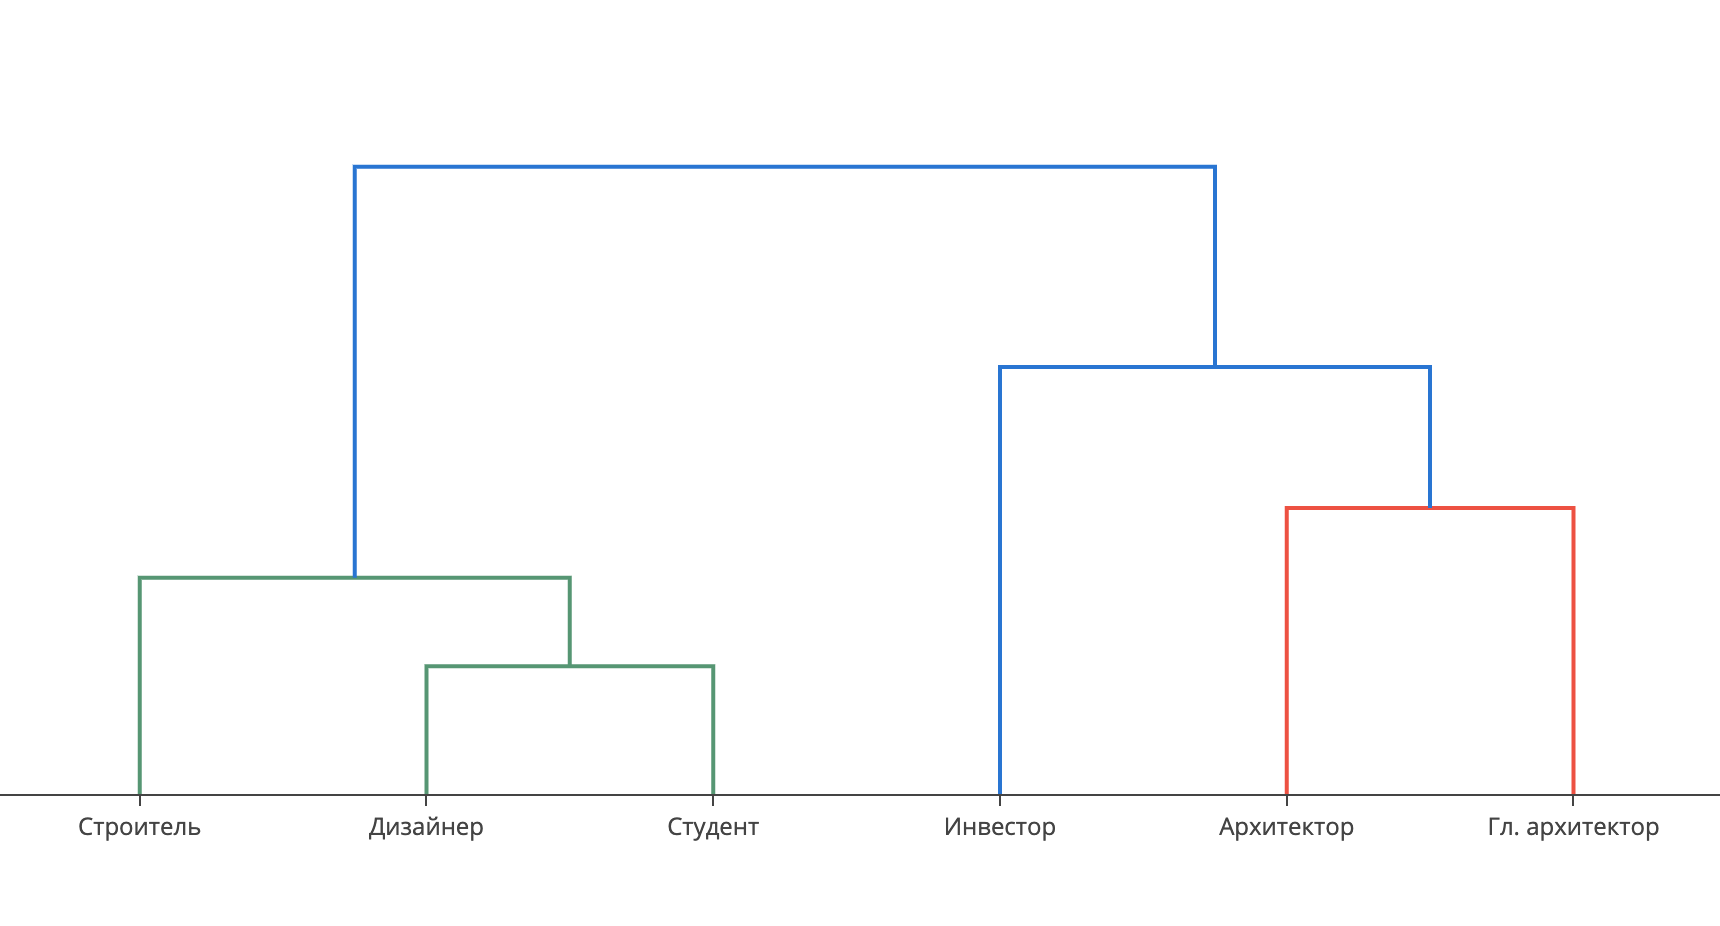
\includegraphics[width=1.0\textwidth]{dendogramm.png}}
\caption{Дендограмма.}
\label{user-stories}
\end{figure}

\subsubsection{Итоговый набор персонажей}

Конечный набор персонажей, которые будут анализироваться в данной работе, представлен ниже:
\begin{itemize}
\item Главный архитектор
\item Архитектор
\item Куратор проекта
\item Строитель
\end{itemize}

Куратором проекта в данном случае является любое лицо, которое желает следить за процессом разработки архитектурных проектов, например, инвестор.

\newpage
\subsection{Действия пользователей}

Описанные в разделе ранее пользователи имеют следующие цели при работе с нашей системой, а также планируют выполнять определенные действия с некоторыми ограничениями.

\subsubsection{Главный архитектор}

\textit{Личные цели:}
\begin{enumerate}
\item Создание крупных архитектурных проектов зданий.
\item Контроль над процессом разработки проекта.
\end{enumerate}
\textit{Действия:}
\begin{enumerate}
\item Начать новый архитектурный проект.
\item Итеративная разработка отдельных частей архитектурной модели.
\item Анализ выполненной командой работы.
\item Управление командами проектирования в различных проектах.
\end{enumerate}
\textit{Требования:}
\begin{enumerate}
\item Масштабируемость системы для поддержки работы большого количества людей.
\item Возможность получить данные проекта в любой выбранный промежуток времени.
\item Создание проектов в едином формате данных (IFC4 или IFC2x3).
\item Доступ к системе из любой точки мира.
\item Возможность предоставить права доступа к выбранному проекту как только на чтение, так и на редактирование.
\end{enumerate}

\subsubsection{Архитектор}

\textit{Личные цели:}
\begin{enumerate}
\item Проектирование сложных архитектурных строений.
\item Обучение на основе истории изменений проекта.
\end{enumerate}
\textit{Действия}
\begin{enumerate}
\item Итеративная разработка отдельных частей архитектурной модели.
\item Анализ выполненной другими членами команды работы над проектом.
\end{enumerate}
\textit{Требования}
\begin{enumerate}
\item Возможность одновременной работы с другими членами команды.
\item Возможность детализированного просмотра изменений проекта.
\item Разработка проектов в едином формате данных.
\item Отказоустойчивость системы.
\end{enumerate}

\subsubsection{Куратор}

\textit{Личные цели:}
\begin{enumerate}
\item Контроль над инвестиционными архитектурными проектами.
\end{enumerate}
\textit{Действия}
\begin{enumerate}
\item Просмотр истории этапов проектирования и строительства архитектурного проекта.
\item Получение детализированного описания изменений в выбранной итерации разработки проекта.
\end{enumerate}
\textit{Требования}
\begin{enumerate}
\item Понятный веб-интерфейс системы.
\item Доступ к системе из любой точки мира.
\item Возможность использования API системы для стороннего проекта.
\item Целостность хранимой информации.
\end{enumerate}

\subsubsection{Строитель}

\textit{Личные цели:}
\begin{enumerate}
\item Планирование строительства на основе функциональных и физических данных архитектурного проекта.
\end{enumerate}
\textit{Действия}
\begin{enumerate}
\item Детальное изучение цифрового контента выбранной версии проекта с целью извлечения важных для строительства характеристик.
\end{enumerate}
\textit{Требования}
\begin{enumerate}
\item Простой веб-интерфейс системы.
\item Получение данных о модели архитектурного объекта в выбранной итерации разработки.
\item Сравнительно недорогая лицензия на использование продукта.
\end{enumerate}

\newpage
\subsection{Карта пользовательских историй}

Итоговый набор пользовательских историй выглядит следующим образом.

\begin{figure}[H]
\center{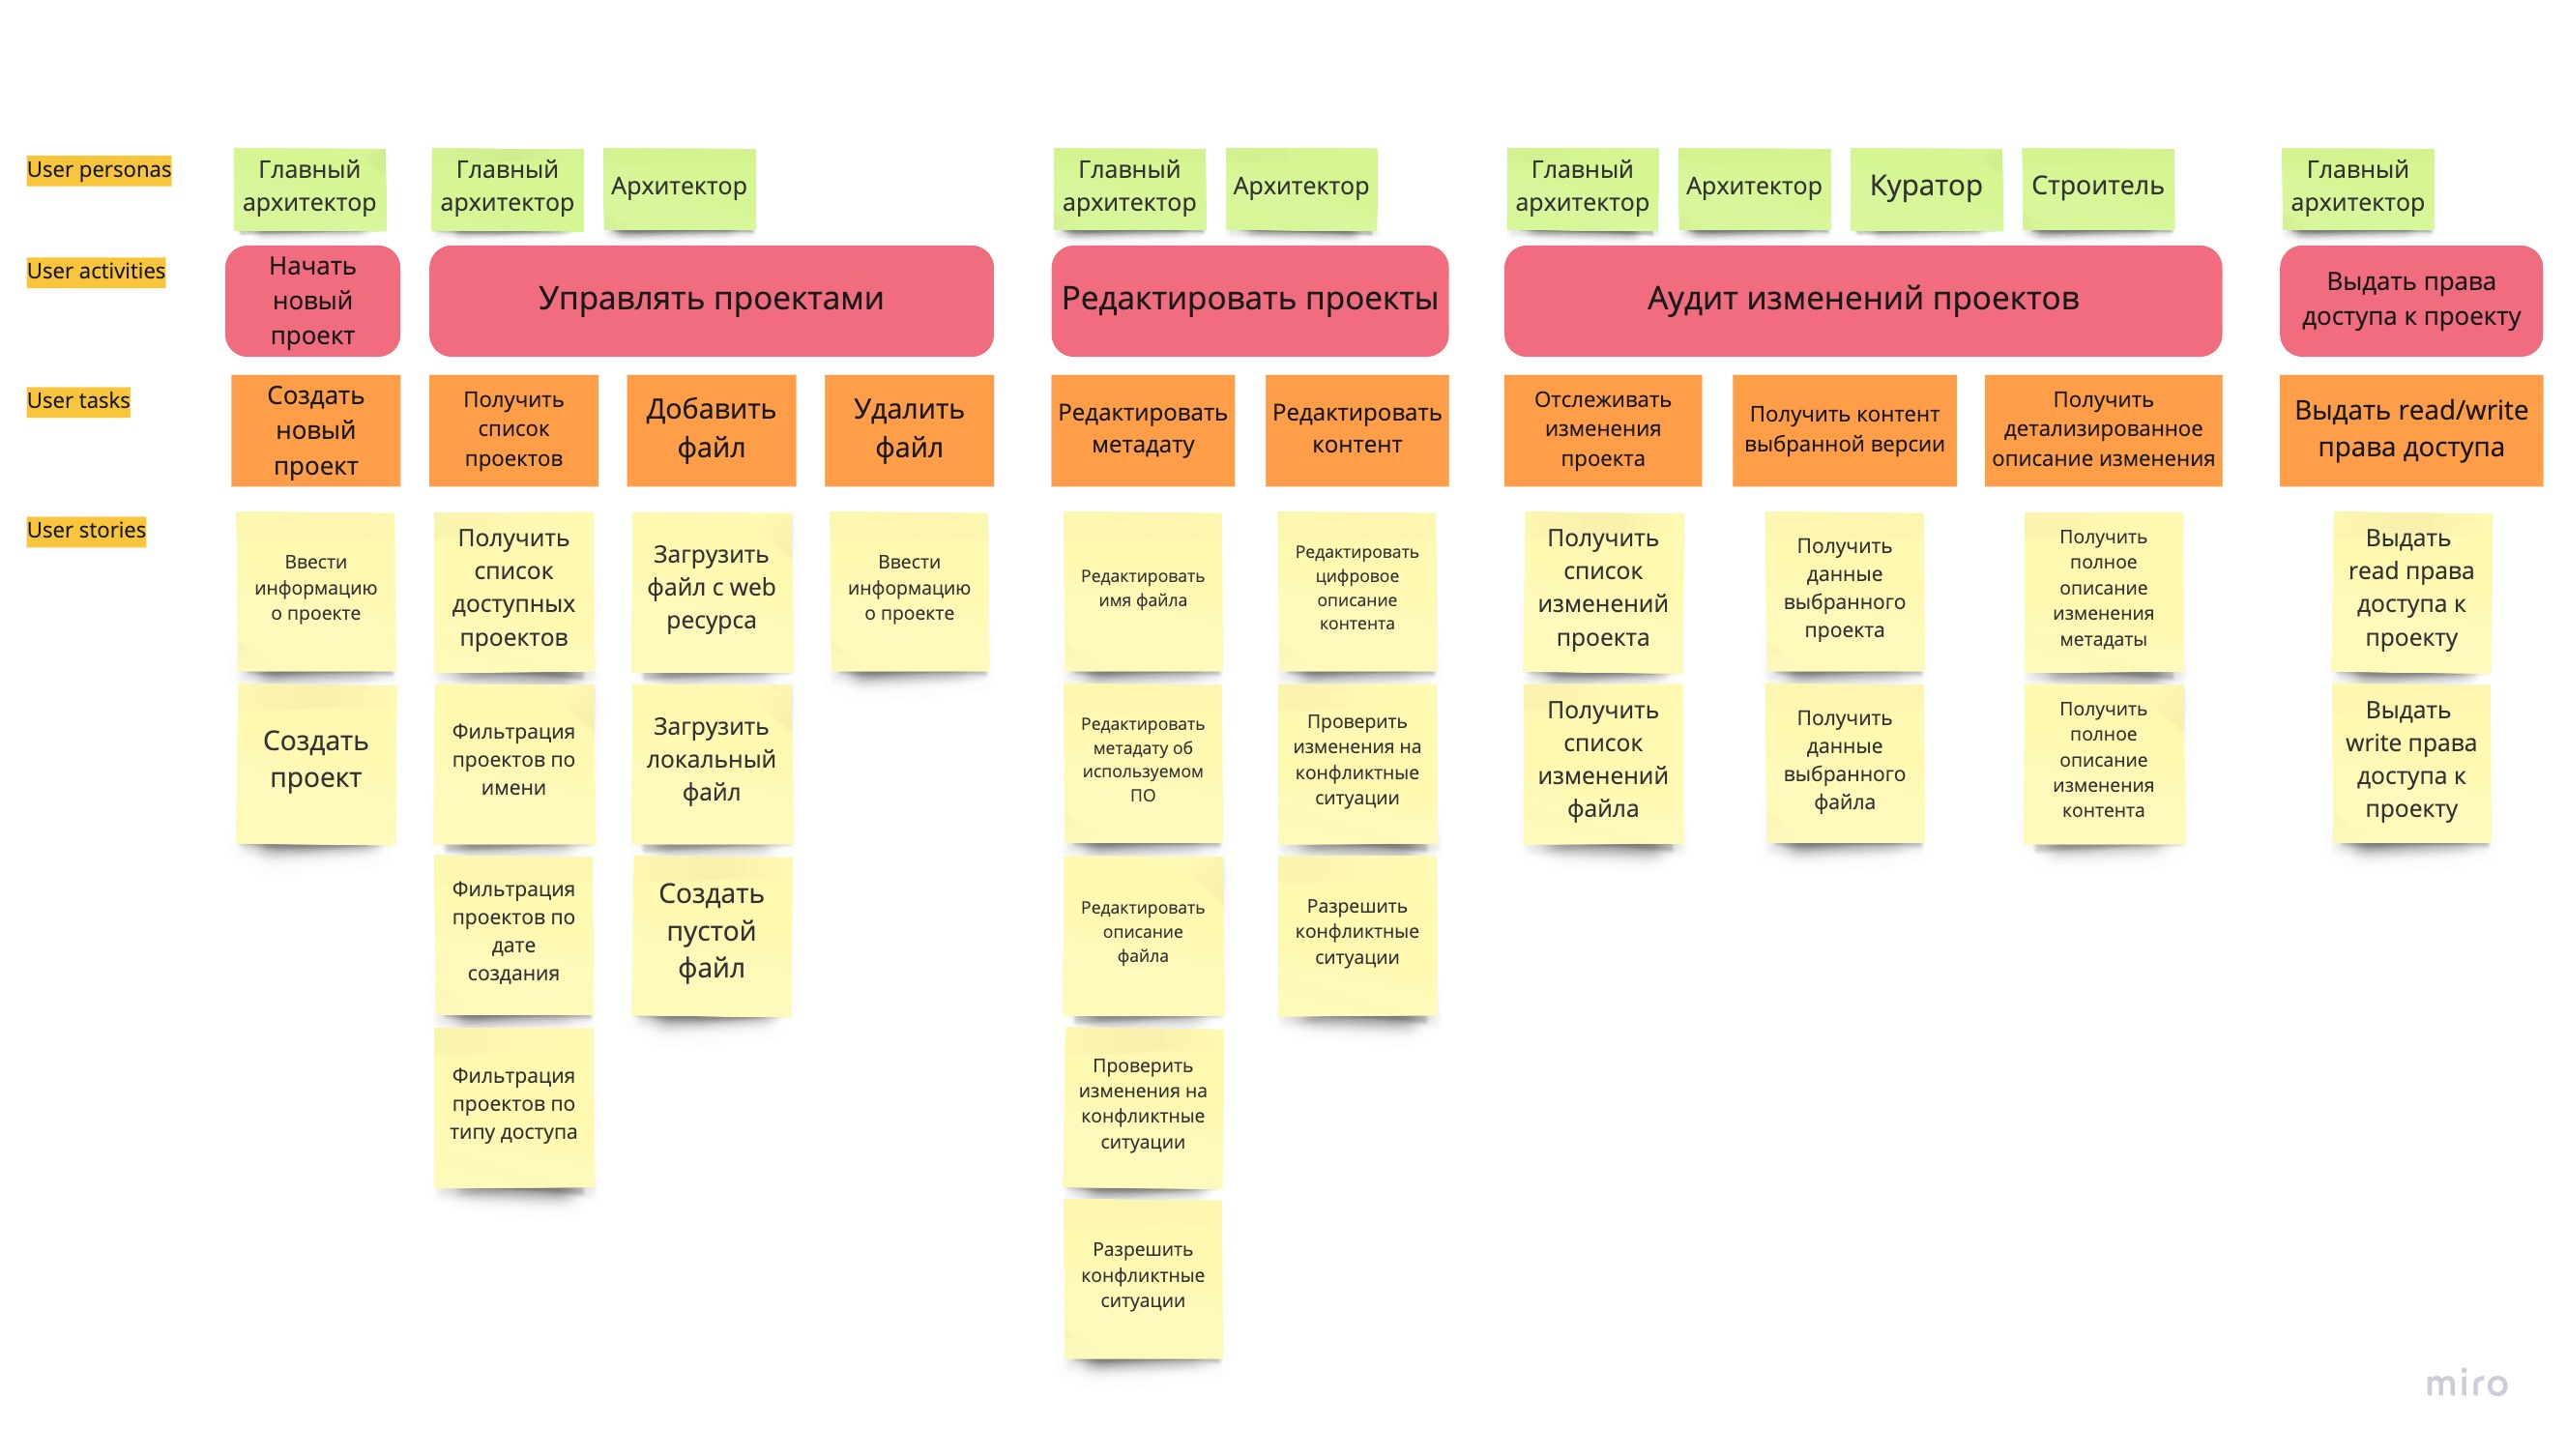
\includegraphics[width=1.0\textwidth]{user-story-mapping.jpg}}
\caption{Пользовательские истории.}
\label{user-stories}
\end{figure}

\newpage
\section{Бизнес-требования}

Бизнес-требования (business requirements) -- информация, в совокупности описывающая потребность, которая инициирует один или больше проектов с целью предоставить решение и получить требуемый конечный результат. В основу бизнес-требований ложатся бизнес-возможности, бизнес-цели, критерии успеха и положение о концепции. \\
Бизнес-требования определяют концепцию решения и границы проекта, в котором оно будет реализовываться. \\
Концепция и границы -- два базовых элемента бизнес-требований. \\ Концепция продукта (product vision) должна кратко описывать конечный продукт, который в свое время должен достигать заданных бизнес-целей. \\
Границы проекта (project scope) показывают, какая часть конечной концепции продукта будет реализована в текущей итерации. \\
В данной работе границы проекта совпадают с концепцией решения. \\
Документ о концепции и границах (vision and scope document) -- единый документ, который включает в себя все бизнес-требования. \\
Далее будут представлены основные пункты этого документа.

\subsection{Исходные данные}

На данный момент архитекторам требуется веб-платформа для одновременной работы с архитектурными проектами без потери данных, которая также предоставляла бы доступ к электронному журналу аудита всех изменений проектов.

\newpage
\subsection{Бизнес-цели}

\begin{table}[H]
\caption {Нефинансовые цели} \label{tab:title}
\begin{center}
\begin{tabular}{ | l | p{14cm} | }
\hline
№ & Цель \\
\hline
Н1 & Разработать веб-платформу для управления жизненным циклом	архитектурных проектов \\
\hline
Н2 & Реализовать возможность одновременного редактирования проектов и разрешения конфликтов в случаях их наличия \\
\hline
Н3 & Реализовать хранение журнала аудита всех изменений проектов и возможность его просмотра \\
\hline
\end{tabular}
\end{center}
\end{table}
 
\subsection{Критерии успеха}

\begin{itemize}
\item Веб-платформа позволяет управлять жизненным циклом архитектурного проекта.
\item Веб-платформе предоставляет возможность просмотра электронного журнала аудита изменений проекта.
\item Веб-платформа позволяет разрешать конфликты, возникающие при одновременном редактировании, без потери данных.
\end {itemize}
 
 \subsection{Положение о концепции проекта}
 
Для пользователей, которым требуется управлять жизненным циклом  архитектурных проектов и иметь возможность отслеживать изменения  во времени, данная работа является веб-платформой, которая будет выступать в качестве единой системы по хранению и изменению архитектурных проектов без потери данных с возможностью просмотра электронного журнала аудита изменений.

\newpage
\section{Ограничения системы}
\subsection{Основные функции}

\begin{enumerate}
\item Просмотр списка доступных пользователю проектов.
\item Создание проекта.
\item Управление правами доступа к проекту.
\item Добавление файлов в проект.
\item Изменение метадаты проекта и его файлов.
\item Удаление файла из проекта.
\item Просмотр контента файла.
\item Редактирование контента файла.
\item Просмотр журнала аудита изменений проекта.
\item Просмотр контента проекта в определенный промежуток времени.
\item Просмотр списка изменений, внесенных в проект в определенный момент времени.
\item Разрешение конфликтных ситуаций при редактировании файлов проекта.
\end {enumerate}

\subsection{Ограничения и исключения}

\begin{itemize}
\item Размер каждого файла должен не превышать 150 Мб (ограничение IFC формата).
\item В данной работе не предполагается возможность создания файлов со связанными между собой BIM представлениями объектов.
\end {itemize}

\newpage

\section{Функции системы}

\begin{enumerate}

\item Просмотр списка проектов \\
Пользователь может просмотреть список доступных ему проектов. Также для поиска проектов имеется возможность фильтрации данных по различным полям.

\begin{table}[H]
\caption {Просмотр списка проектов} \label{tab:title}
\begin{center}
\begin{tabular}{| p{2.5cm}  | p{11.5cm} |}
\hline
\multicolumn{2}{ | l | }{Функциональные требования:} \\
\hline
ПСПФ1 & Система должна предоставить список всех проектов по заданным фильтрам.  \\
\hline
ПСПФ2 & Записи проектов должны содержать следующую информацию: имя, описание проекта, даты создания и последнего изменения, имя владельца, а также краткую информацию о файлах. \\
\hline
\multicolumn{2}{ | l | }{Нефункциональные требования:} \\
\hline
ПСПН1 & Пользователю отображаются только те проекты, владельцем которых он является, или к которым он имеет доступ на чтение или редактирование .\\
\hline
\end{tabular}
\end{center}
\end{table}

\item Создание проекта \\
Создание проекта с возможностью указания его названия и полного описания.

\begin{table}[H]
\caption {Создание проекта} \label{tab:title}
\begin{center}
\begin{tabular}{| p{2.5cm}  | p{11.5cm} |}
\hline
\multicolumn{2}{ | l | }{Функциональные требования:} \\
\hline
СПФ1 & При создании проекта система должна предоставить пользователю идентификатор, по которому он теперь сможет работать с только что созданным проектом. \\
\hline
СПФ2 & При создании проекта система предоставляет пользователю возможность ввести имя и описание нового проекта. \\
\hline
\end{tabular}
\end{center}
\end{table}

\item Управление правами доступа к проекту \\
Предоставление доступа либо на чтение, либо на редактирование к проекту другим пользователям.

\begin{table}[H]
\caption {Управление правами доступа} \label{tab:title}
\begin{center}
\begin{tabular}{| p{2.5cm}  | p{11.5cm} |}
\hline
\multicolumn{2}{ | l | }{Функциональные требования:} \\
\hline
ПДФ1 & Каждому пользователю можно выдать права доступа к проекту. \\
\hline
\multicolumn{2}{ | l | }{Нефункциональные требования:} \\
\hline
ПДН1 & Права пользователей подразделяются на чтение, редактирование. Права на чтение подразумевают только просмотр всех данных проекта и его изменений. Права на редактирование включают в себя права на чтение, а также возможность управлять жизненным циклом проекта. \\
\hline
ПДН2 & Только владелец проекта имеет возможность предоставлять какие-либо права доступа к проекту. \\
\hline
ПДН3 & По умолчанию новый проект доступен только его владельцу. \\
\hline
\end{tabular}
\end{center}
\end{table}

\item Добавление файлов в проект \\
В уже созданный проект происходит добавление нового файла с контентом. Загружаться данные могут как по ссылке, так и сам файл с данными. Есть возможность создать пустой файл. \\

\begin{table}[H]
\caption {Добавление файлов в проект} \label{tab:title}
\begin{center}
\begin{tabular}{| p{2.5cm}  | p{11.5cm} |}
\hline
\multicolumn{2}{ | l | }{Функциональные требования:} \\
\hline
ДФФ1 & При невозможности загрузить данные система должна оповестить об этом пользователя (с указанием причины). \\
\hline
ДФФ2 & Система предоставляет возможность загрузить файл с другого веб-источника данных. \\
\hline
ДФФ3 & Система предоставляет возможность загрузить локальный файл с персонального компьютера пользователя. \\
\hline
ДФФ4 & Система предоставляет возможность создать полностью пустой файл. \\
\hline
\multicolumn{2}{ | l | }{Требования к данным:} \\
\hline
ДФД1 & Формат загружаемых данных должен соответствовать стандарту IFC .\\
\hline
ДФД2 & Максимальный размер загружаемых данных - 150 Мб. \\
\hline
\end{tabular}
\end{center}
\end{table}

\item Редактирование контента файла \\
Пользователь имеет возможность изменить контент неудаленных файлов в проектах. \\

\begin{table}[H]
\caption {Редактирование контента файла} \label{tab:title}
\begin{center}
\begin{tabular}{| p{2.5cm}  | p{11.5cm} |}
\hline
\multicolumn{2}{ | l | }{Функциональные требования:} \\
\hline
РКФ1 & После внесения изменений в контент текущей версии файла система должна проверить корректность данного изменения и оповестить пользователя либо о невозможности выполнения, либо об успешности операции \\
\hline
РКФ2 & После внесения изменений в контент файла система должна обновить историю проекта \\
\hline
\multicolumn{2}{ | l | }{Нефункциональные требования:} \\
\hline
РКН1 & Вносить изменения разрешается только в неудаленные файлы \\
\hline
\end{tabular}
\end{center}
\end{table}

\end {enumerate}


\newpage
\section{Описание системы}


\newpage
\section{Описание алгоритмов}


\newpage
\section{Инфраструктура веб-платформы}


\newpage
\section{Характеристики качества}


\newpage
\chapter{Заключение}

\begin{thebibliography}{1}
{\small
\bibitem{BUILDING_GROWTH_RATE} {\it GlobalData.}
\textbf{Global construction output growth to reach 3.4\% in 2019} // Публикация на www.globaldata.com. 11 April 2019.
\bibitem{BUILDING_SOFTWARE} \textit{Ar. Mustakeem Raza Khan, Prof. S.K Gupta, Ar. Rakesh Kumar.}
\textbf{Role of Computer’s Technology: Architectural Design} // International Journal for Research in Applied Science \& Engineering Technology (IJRASET)
\bibitem{BIM_FUTURE} {\it Karen M. Kensek, Douglas E. Noble.}
\textbf{Building Information Modeling: BIM in Current and Future Practice (1st ed.)} // 2014 Hoboken, New Jersey: John Wiley
\bibitem{BIM_ADVANTAGES} {\it Arayici, Y, Coates, P, Koskela, LJ, Kagioglou, M, Usher, C.}
\textbf{Technology adoption in the BIM implementation for lean architectural practice)} // Technology adoption in the BIM implementation for lean architectural practice, Automation in Construction, 2011. pp. 189-195.
\bibitem{BIM_USAGE} {\it McAuley, B., Hore, A. and West R.}
\textbf{BICP Global BIM Study - Lessons for Ireland’s BIM Programme} // Construction IT Alliance (CitA), 2017
\bibitem{BIM_UK} {\it UK Government.}
\textbf{Level 3 Building Information Modelling - Strategic Plan} // Digital Built Britain, February 2015
\bibitem{BIM_RUSSIA} {\it Президент Российской Федерации Путин В. В.}
\textbf{Поручение ПР-1235} // 19.07.2018.
}
\end{thebibliography}

\end{document}
